
\documentclass{exam}

\usepackage{siunitx} 
\usepackage{graphicx}
\usepackage[fleqn]{amsmath}
\usepackage{cancel}
\usepackage{polynom}
\usepackage{float}
\usepackage{mdwlist}
\usepackage{booktabs}
\usepackage{cancel}
\usepackage{polynom}
\usepackage{caption}

\newcommand{\degree}{\ensuremath{^\circ}} 
\everymath{\displaystyle}

% \begin{figure}[H]
%   \centering
%   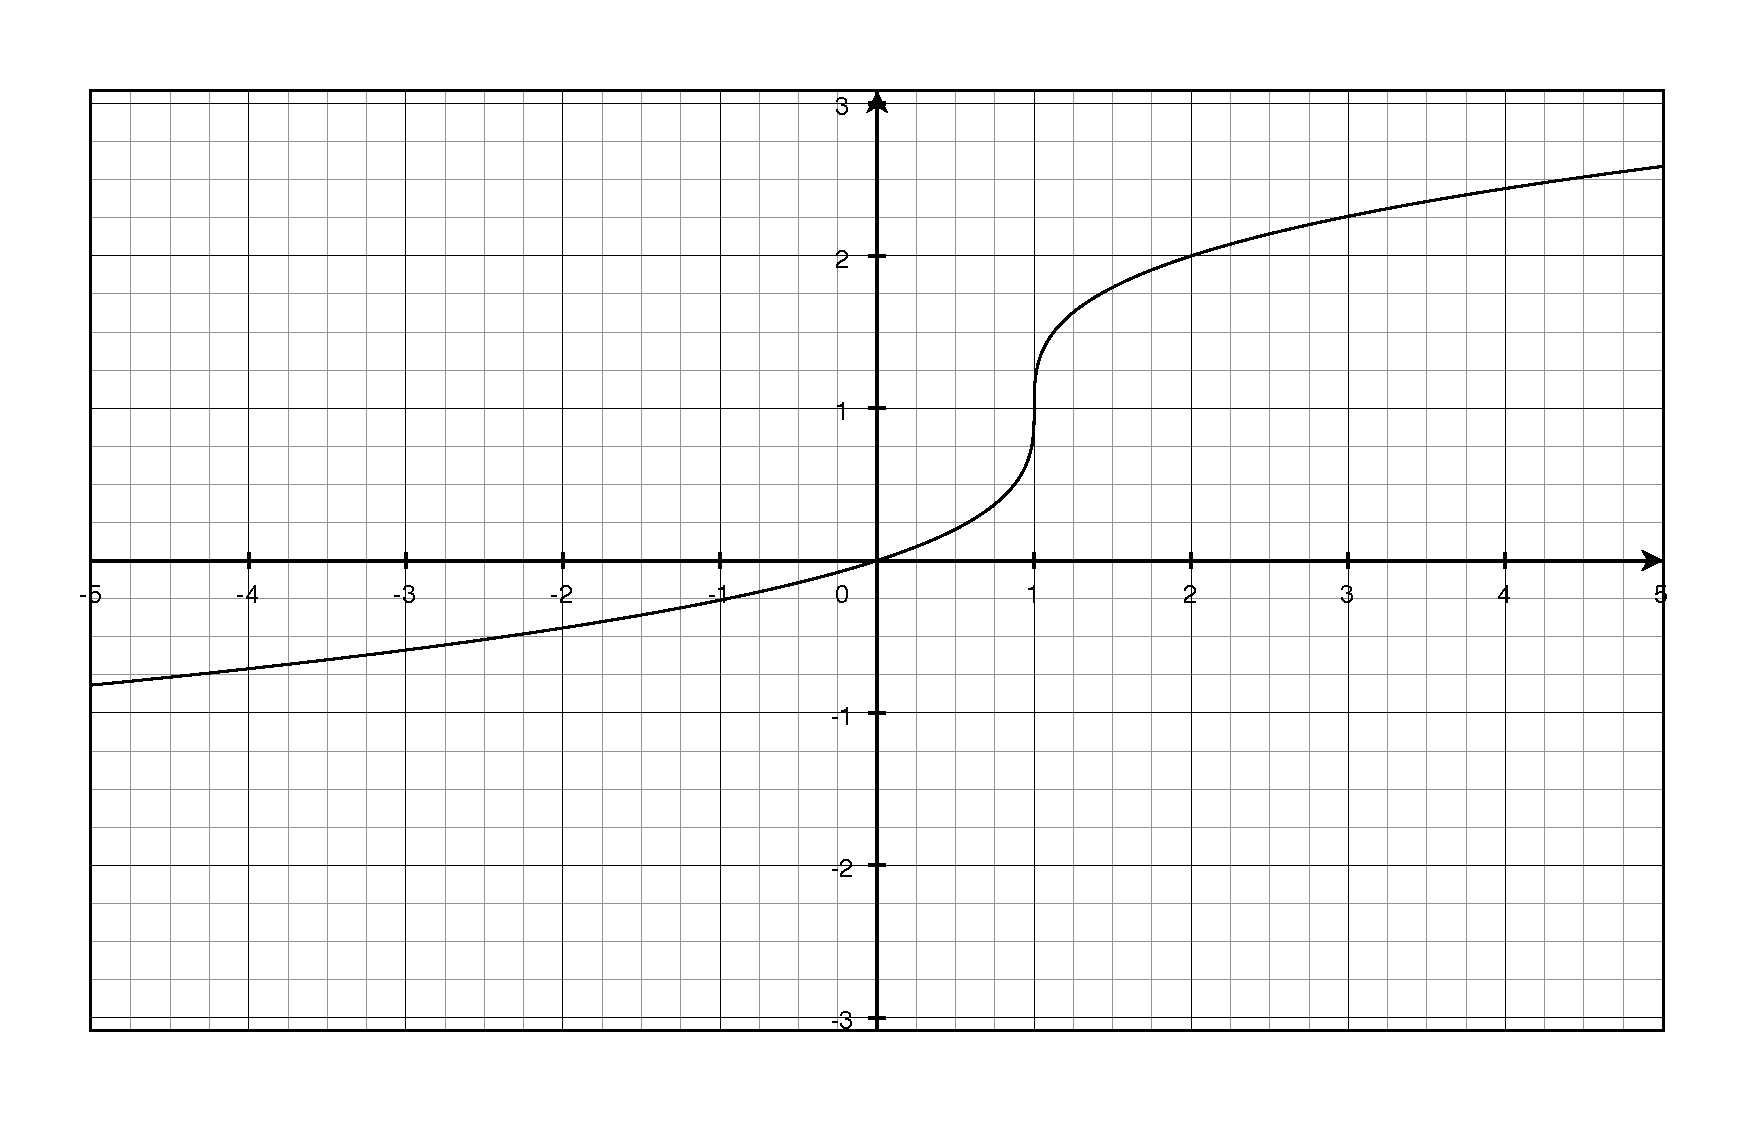
\includegraphics[scale=.3]{question7.eps}
%   \caption*{Question 7}
% \end{figure}

% \begin{tabular}{cc}
% \toprule
% period & amplitude \\
% \midrule
%   $\pi$ & $2$ \\
% \bottomrule
% \end{tabular}

\textwidth 6.5 in

\printanswers

\ifprintanswers 
\usepackage{2in1, lscape} 
\fi

\title{Math 263a \\ Homework One}
\date{January 11, 2011}

\begin{document}

\maketitle

\section{Homework}

\begin{itemize*}
  \item Read Section 2.1
  \item pp 47-49: 1, 10-12, 15-16, 19, 21-22, 24, 27, 32
\end{itemize*}

\section{Extra Credit}

pp 47-49: 36 and 39

\ifprintanswers
\begin{description}
\item[36]
To figure out the area, we first need to find the height.  The height goes from one vertex to the middle of the opposite
side.  If we let $s$ be the length of a side, we can use the Pythagorean theorem to find the height:

\begin{align*}
  \left( \frac{s}{2} \right)^2 + h^2 &= s^2 \\
  h^2 &= s^2 - \frac{s^2}{4} \\
  h &= \frac{\sqrt{3}}{2} s \\
\end{align*}

Now we can find the area as a function of side length, since 
\[
  A = \frac{1}{2} bh
\]

\begin{align*}
  A(s) &= \frac{1}{2} \cdot s \cdot \frac{\sqrt{3}}{2} s \\
       &= \frac{\sqrt{3}}{4} s^2 \\
\end{align*}


We really want a function in terms of the perimeter.  Each side is one third of the perimeter, so the final
function is:
\begin{align*}
  A(p) &= \frac{\sqrt{3}}{4} \left( \frac{p}{3} \right)^2 \\
       &= \frac{\sqrt{3}}{36} p^2 \\
\end{align*}

\item[39]
The area of the track is the area of the semicircles at the ends plus the area of the rectangle in the middle.  

The area of the two semicircles combined is:
\[
  A_{ends} = \pi \left(\frac{d}{2}\right)^2 = \frac{\pi d^2}{4}
\]

The circumference of the two semicircles is $\pi d$.  So the outside length of one side of the rectangle is 
\[
  \frac{1}{2} (1 - \pi d)
\]

The inside length of one side of the rectangle is the diameter of the circular ends.  So the area of the rectangle is:
\[
  A_{rectangle} = \frac{1}{2} (1 - \pi d) \cdot d = \frac{d - \pi d^2}{2}
\]

The total area is:
\begin{align*}
  A_{total} &= A_{ends} + A_{rectangle} \\
           &= \frac{\pi d^2}{4} + \frac{d - \pi d^2}{2} \\
           &= \frac{\pi d^2 + 2d - 2 \pi d^2}{4} \\
           &= \frac{2d - \pi d^2}{4} \\
\end{align*}
The smallest circle you can have with a circumference of 1 mile is:
\begin{align*}
  \pi d &= 1 \\
  d &= \frac{1}{\pi} \\
\end{align*}
This would make the straight parts of the track go away.  With smaller diameter circles, you leave some room for the
straight part of the track.  Since we want to have circles on each end and at least a minimal straight part, the
diameter must be in the range:
\[
  d < \frac{1}{\pi}
\]

\end{description}

\section{Questions}

\begin{description}

\item[1]
\begin{description}
\item[a] $f(1) = 0$
\item[b] $f(-2) = -3$
\item[c] $f(0) = 1$
\item[d] $f(k) = 1 - k^2$
\item[e] $f(-5) = -24$
\item[f] $f\left(\frac{1}{4}\right) = \frac{15}{16}$
\item[g] $f(3t) = 1 - 9t^2$
\item[h] $f(2x) = 1 - 4x^2$
\item[i] $f \left( \frac{1}{t} \right) = 1 - \frac{1}{t^2}$
\end{description}

\item[10]
You can draw a vertical line which intersects the graph in more than one point for the graphs of {\em a} and {\em c}, so
these two are not functions.  The other two are functions. 

\item[11]
\begin{align*}
  \frac{f(a+h) - f(a)}{h} &= \frac{2(a+h)^2 - 1 - (2a^2 - 1)}{h} \\
                          &= \frac{2(a^2 + 2ah + h^2) - 1 - 2a^2 + 1}{h} \\
                          &= \frac{2a^2 + 4ah + 2h^2 - 1 - 2a^2 + 1}{h} \\
                          &= \frac{4ah + 2h^2}{h} \\
                          &= 4a + 2h \\
\end{align*}

\item[12]
\begin{align*}
  \frac{F(a+h) - F(a)}{h} &= \frac{4(a+h)^3 - 4a^3}{h} \\
                          &= \frac{4(a+h)(a^2 + 2ah + h^2) - 4a^3}{h} \\
                          &= \frac{4(a^3 + 2a^2h + ah^2 + a^2h + 2ah^2 + h^3) - 4a^3}{h} \\
                          &= \frac{4(a^3 + 3a^2h + 3ah^2 + h^3) - 4a^3}{h} \\
                          &= \frac{4a^3 + 12a^2h + 12ah^2 + 4h^3 - 4a^3}{h} \\
                          &= \frac{12a^2h + 12ah^2 + 4h^3}{h} \\
                          &= 12a^2 + 12ah + 4h^2 \\
\end{align*}

\item[15]
\begin{description}
\item[a] 
\begin{align*}
  2z + 3 &\geq 0 \\
  2z &\geq -3 \\
  z &\geq -\frac{3}{2} \\
\end{align*}

\item[b] 
\begin{align*}
  4v - 1 &\neq 0 \\
  4v &\neq 1 \\
  v &\neq \frac{1}{4} \\
\end{align*}

\item[c]
\begin{align*}
  x^2 - 9 &\geq 0 \\
  x^2 &\geq 9 \\
  |x| &\geq 3 \\
\end{align*}

\item[d]
\begin{align*}
  625 - y^4 &\geq 0 \\
  y^4 &\leq 625 \\
  |y| &\leq 5 \\
\end{align*}

\end{description}

\item[16]
\item[a]
\begin{align*}
  x^2 - x - 6 &\neq 0 \\
  (x-3)(x+2) &\neq 0 \\
\\
  x \neq 3 \text{ and } x \neq -2 \\
\end{align*}

\item[b]
\begin{align*}
  y + 1 &> 0 \\
  y &> -1 \\
\end{align*}

\item[c]
Any real number will work.

\item[d]
Any real number will work.

\item[19]
\[
  f(-x) = -2x + 1 \neq f(x) \neq -f(x)
\]

Neither even nor odd.

\begin{figure}[H]
  \centering
  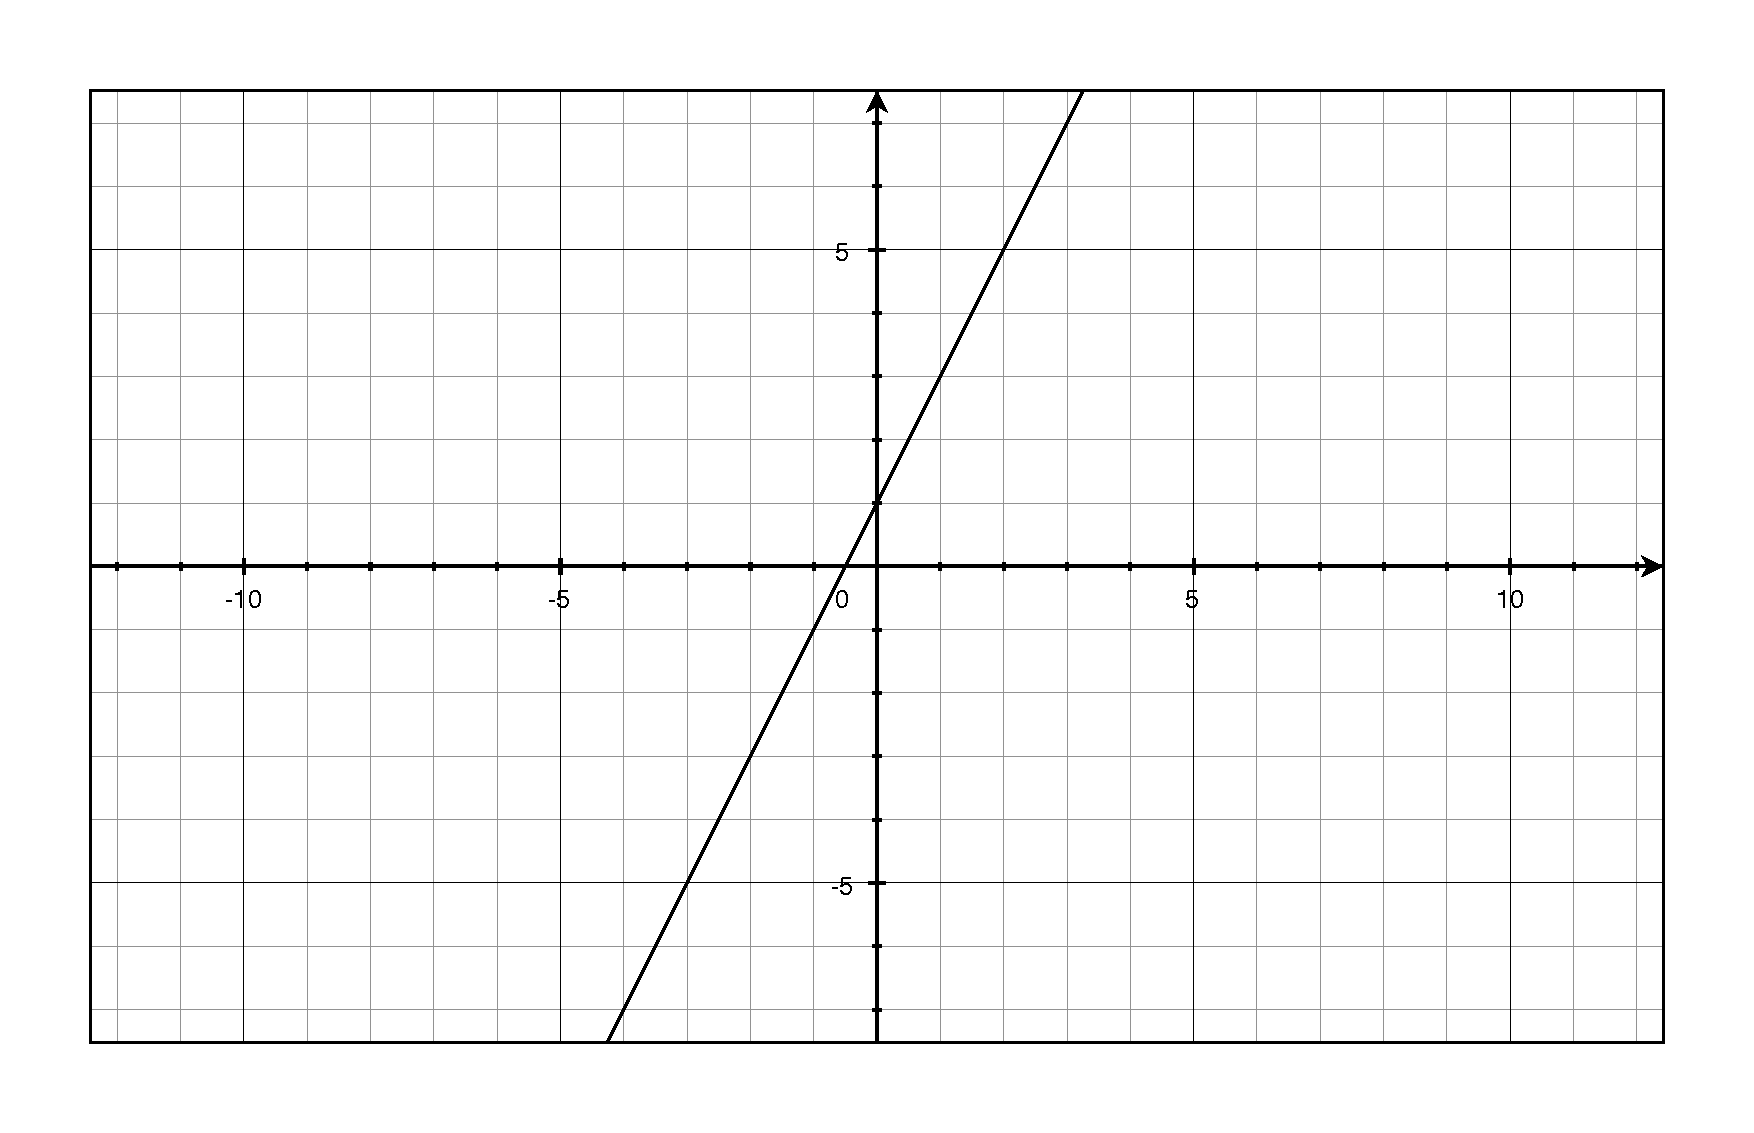
\includegraphics[scale=.3]{question_19.eps}
  \caption*{Question 19}
\end{figure}

\item[21]
\[
  f(-x) = 3x^2 -2x - 1 \neq f(x) \neq -f(x)
\]

Neither even nor odd.

\begin{figure}[H]
  \centering
  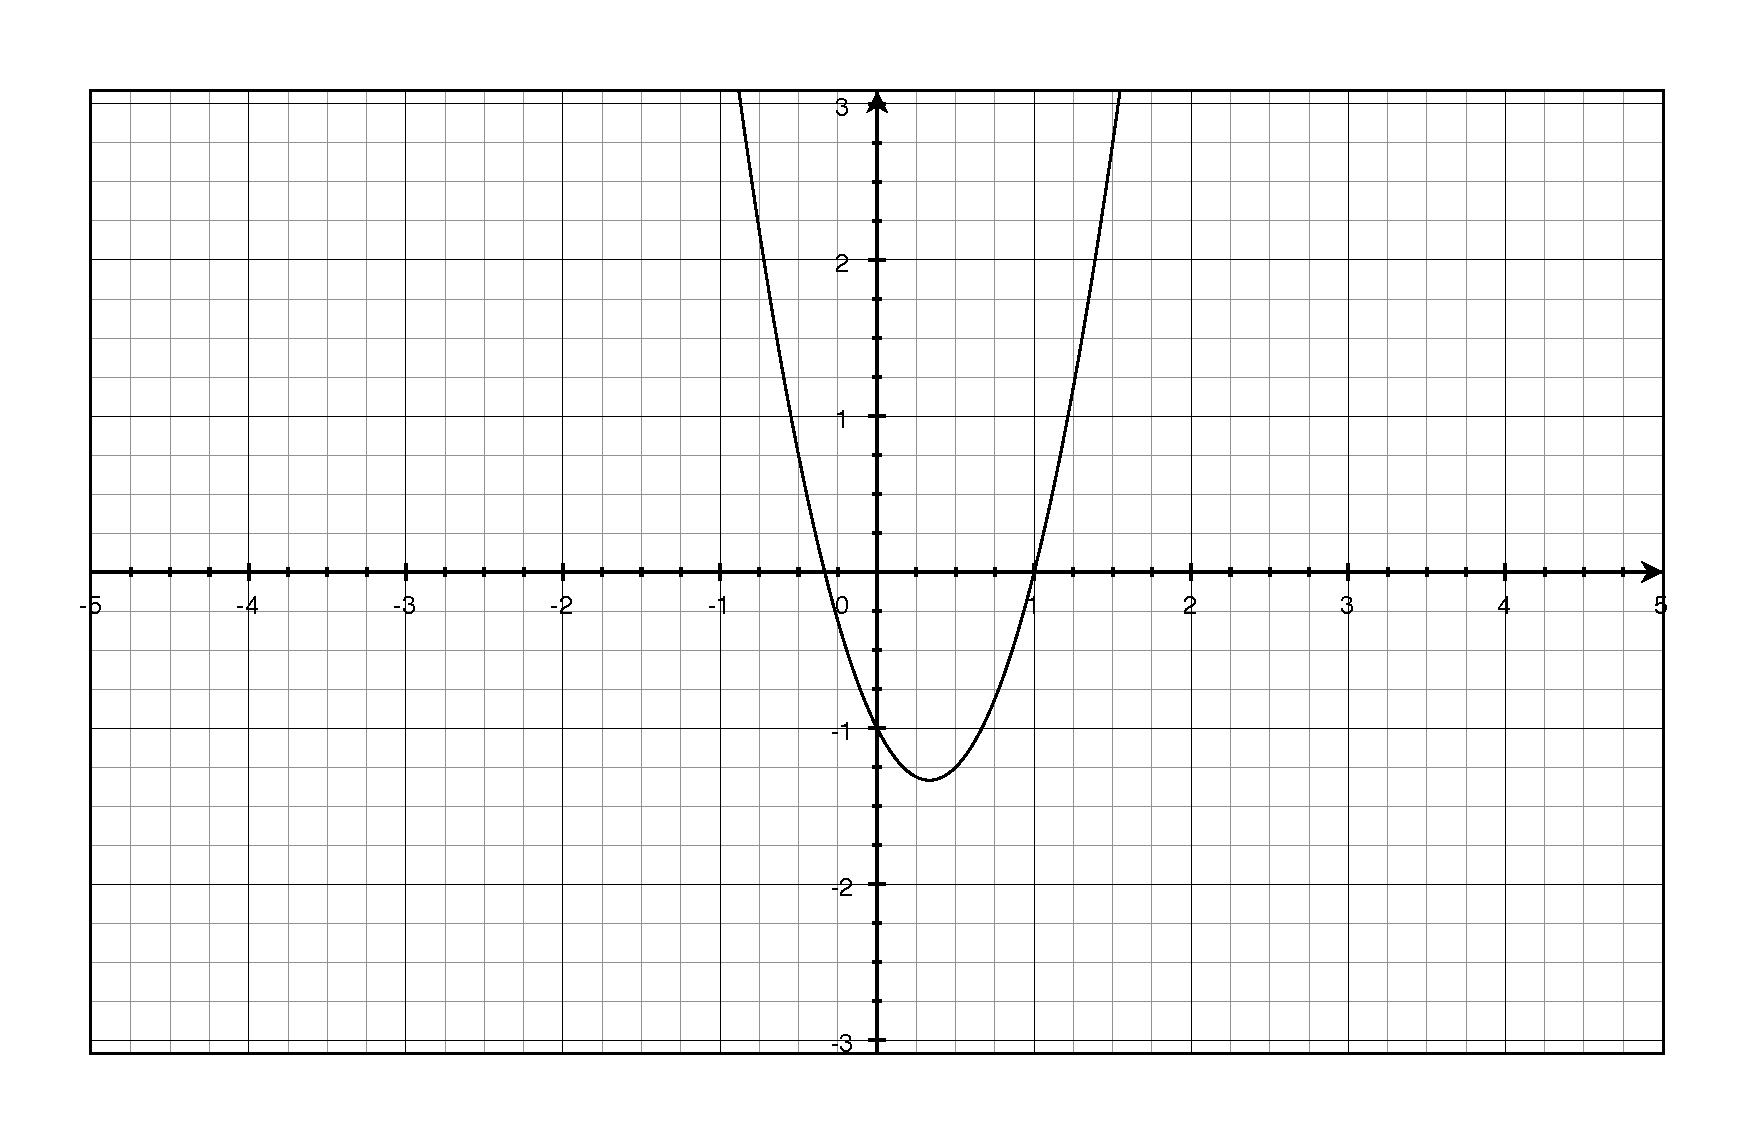
\includegraphics[scale=.3]{question_21.eps}
  \caption*{Question 21}
\end{figure}

\item[22]
\[
  f(-u) = -\frac{u^3}{8} = -f(u)
\]

Odd.

\begin{figure}[H]
  \centering
  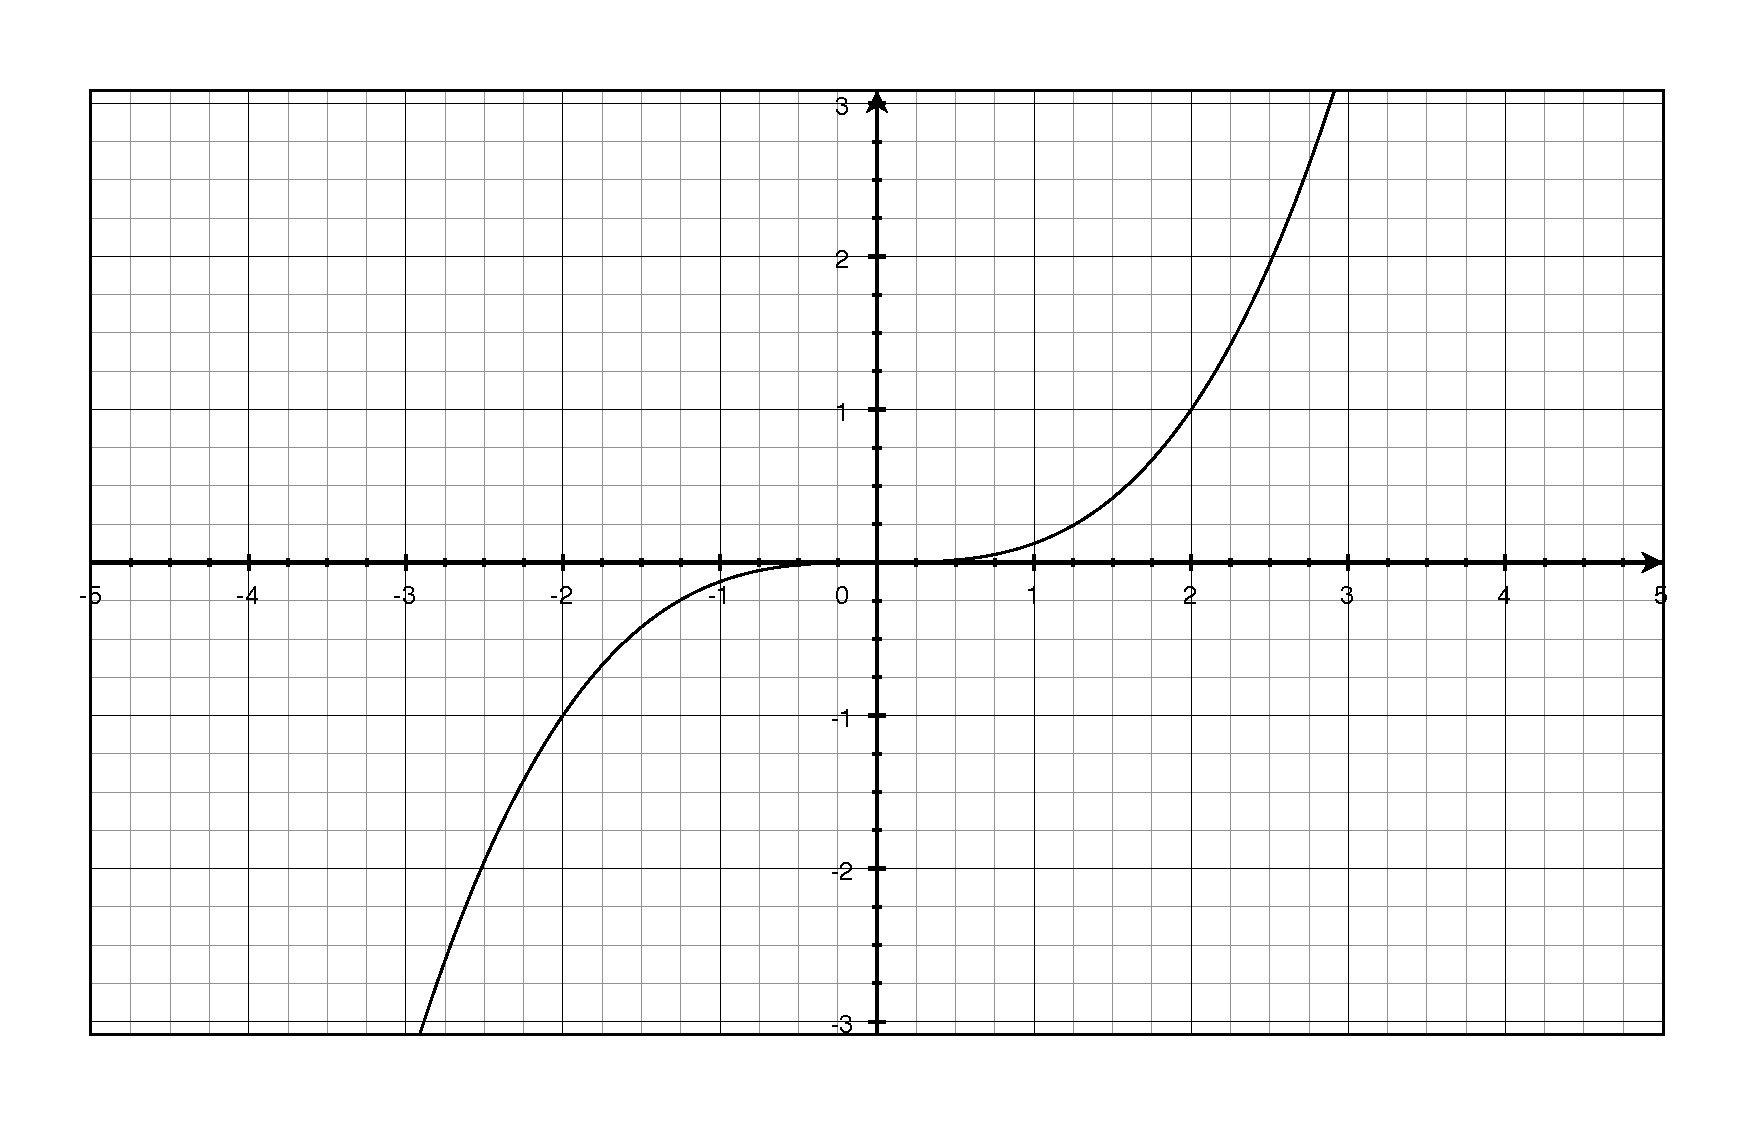
\includegraphics[scale=.3]{question_22.eps}
  \caption*{Question 22}
\end{figure}

\item[24]
\[
  f(-z) = \frac{-2z+1}{-z-1} \neq f(z) \neq -f(z)
\]

Neither even nor odd.

Since the degree of the numerator and denominator is the same, there is a horizontal asymptote at 
\[
  y = \frac{2}{1} = 2
\]

The numerator is zero at $z = 1$, so there is a vertical asymptote at $z = 1$

\begin{figure}[H]
  \centering
  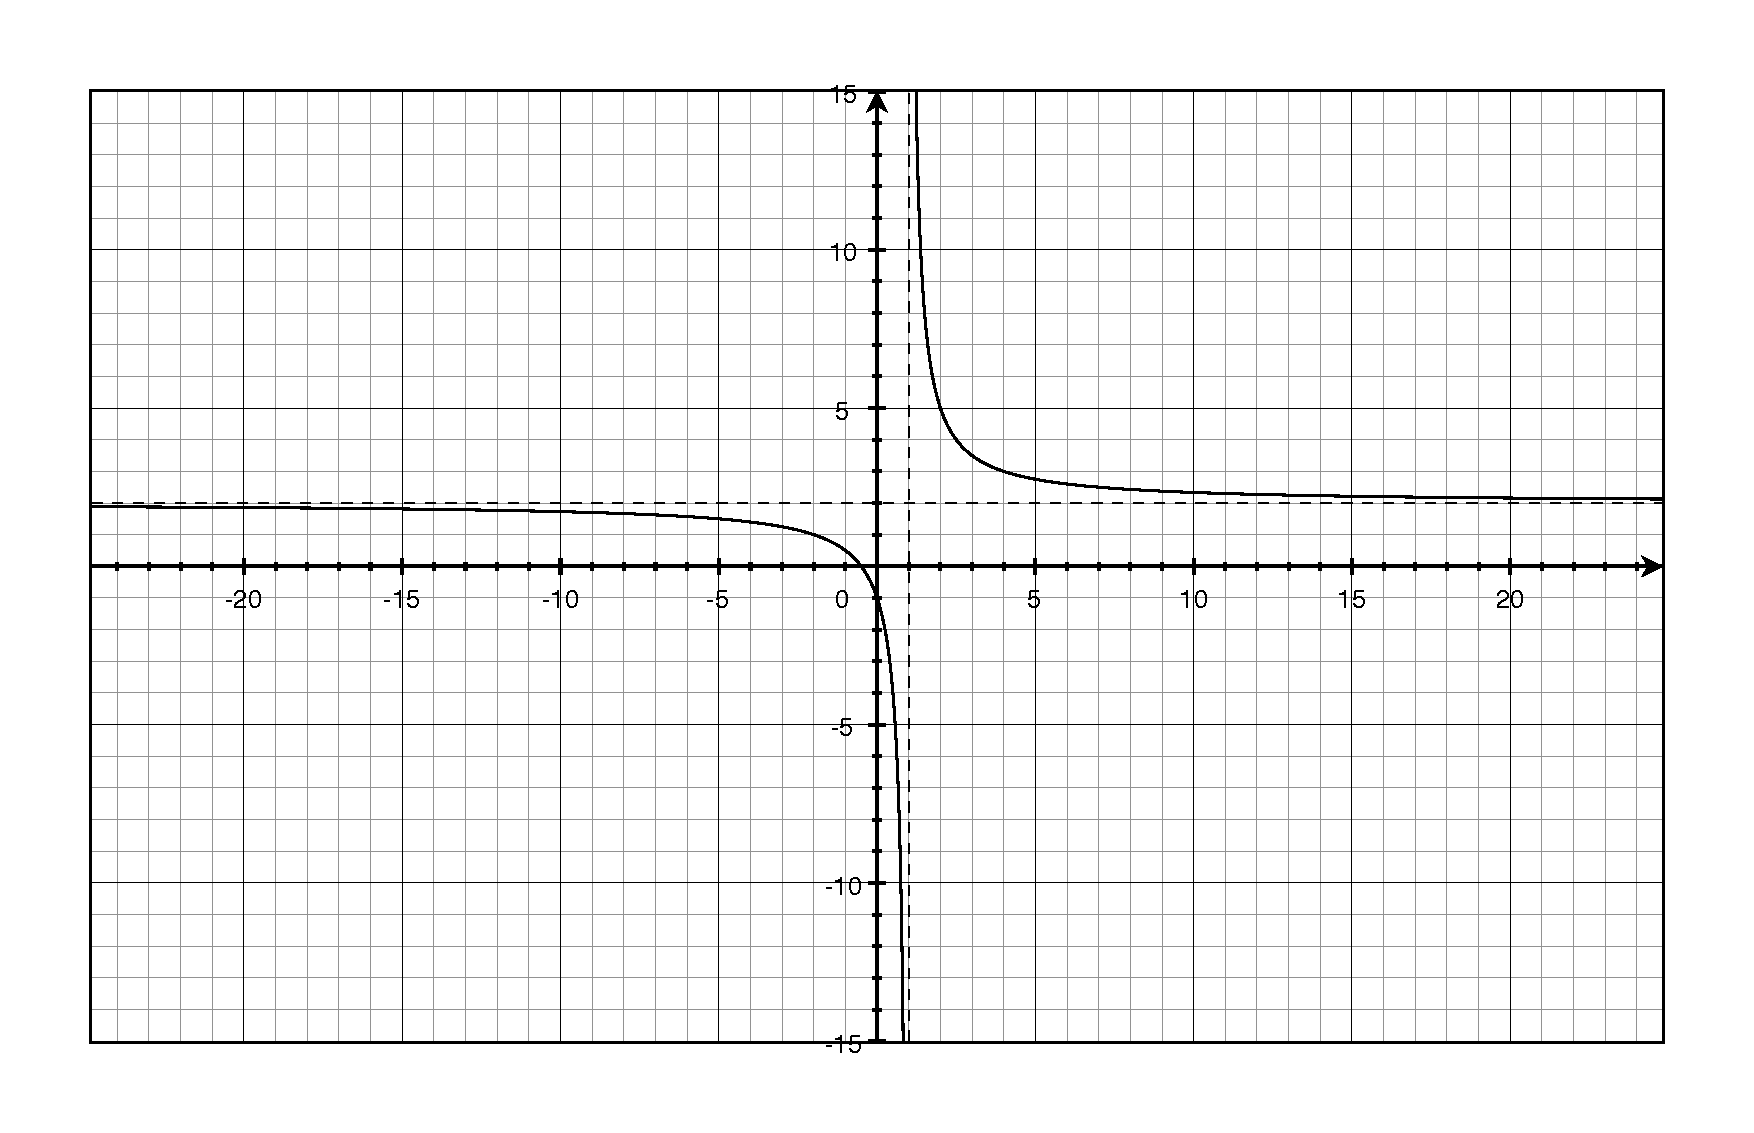
\includegraphics[scale=.3]{question_24.eps}
  \caption*{Question 24}
\end{figure}


\item[27]
\[
  f(-x) = |-2x| = |2x| = f(x) 
\]

Even.

\begin{figure}[H]
  \centering
  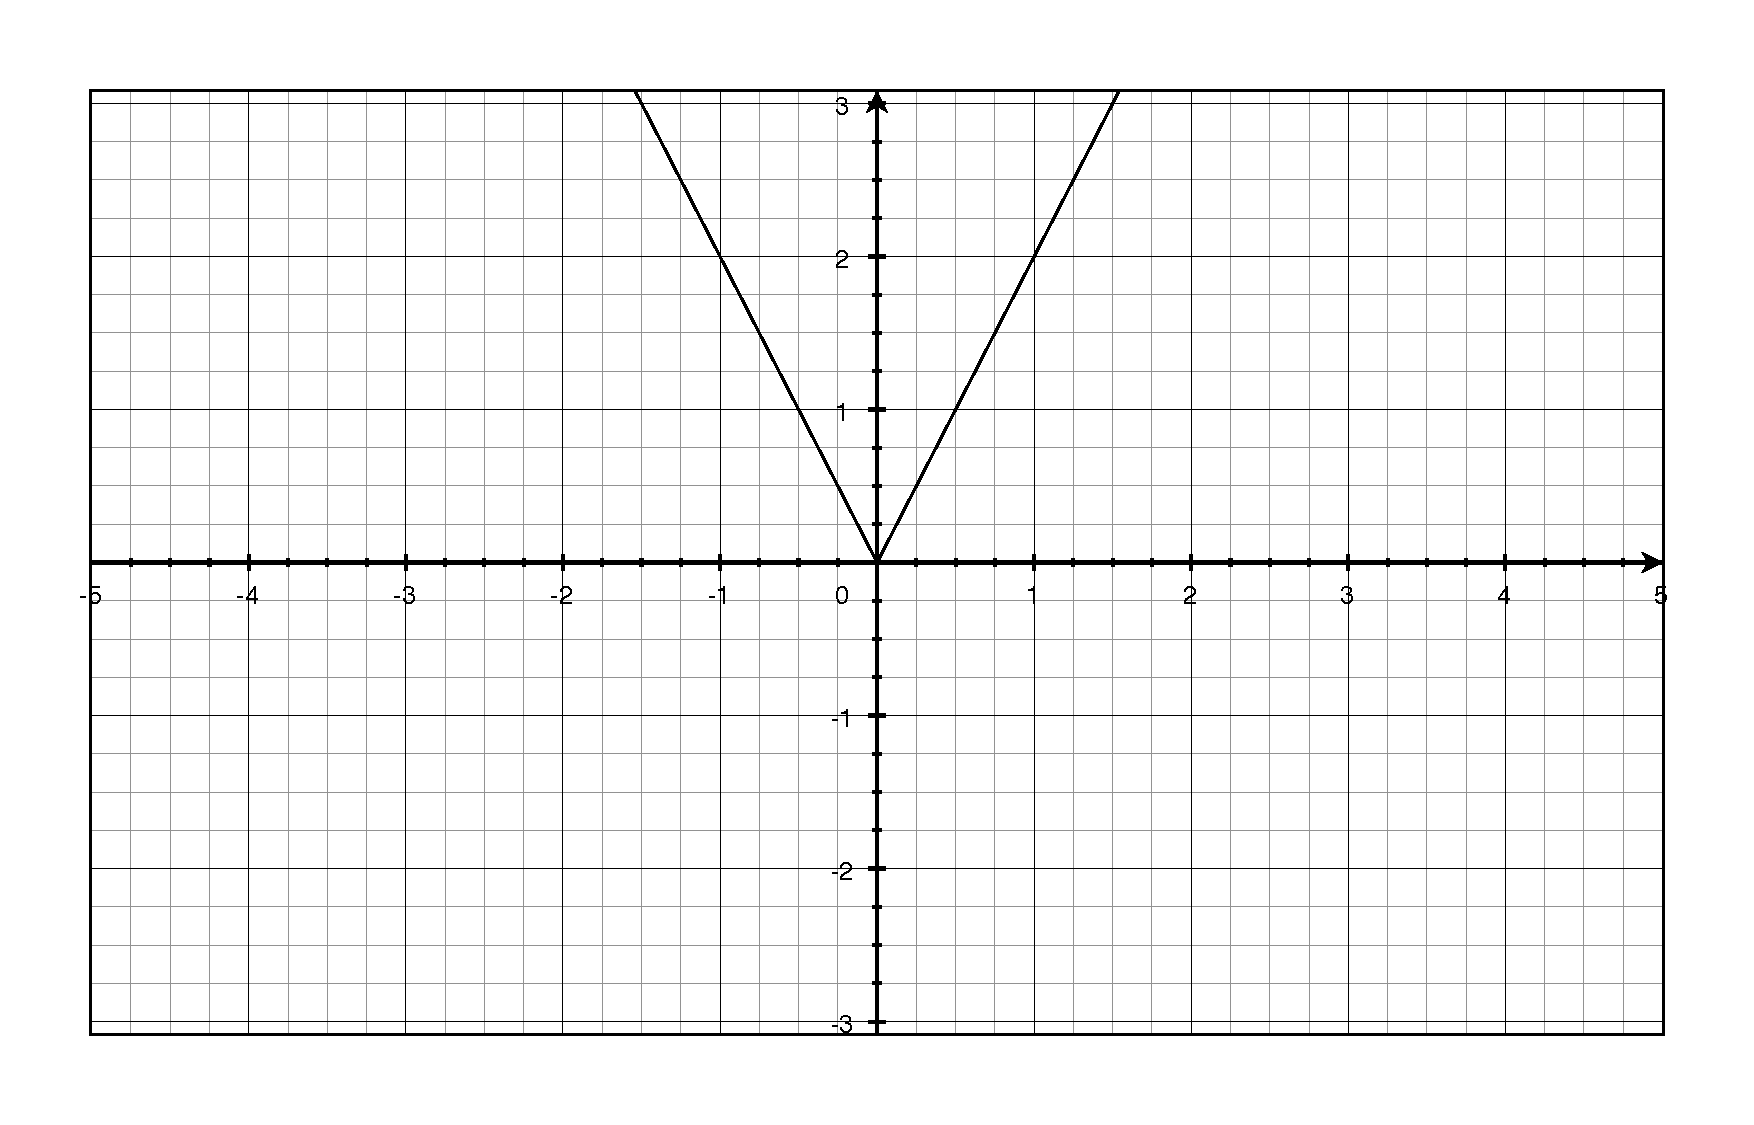
\includegraphics[scale=.3]{question_27.eps}
  \caption*{Question 27}
\end{figure}

\item[32]
One part of the function is even and the other part is odd, so the function as a whole is neither even nor odd. 

\begin{figure}[H]
  \centering
  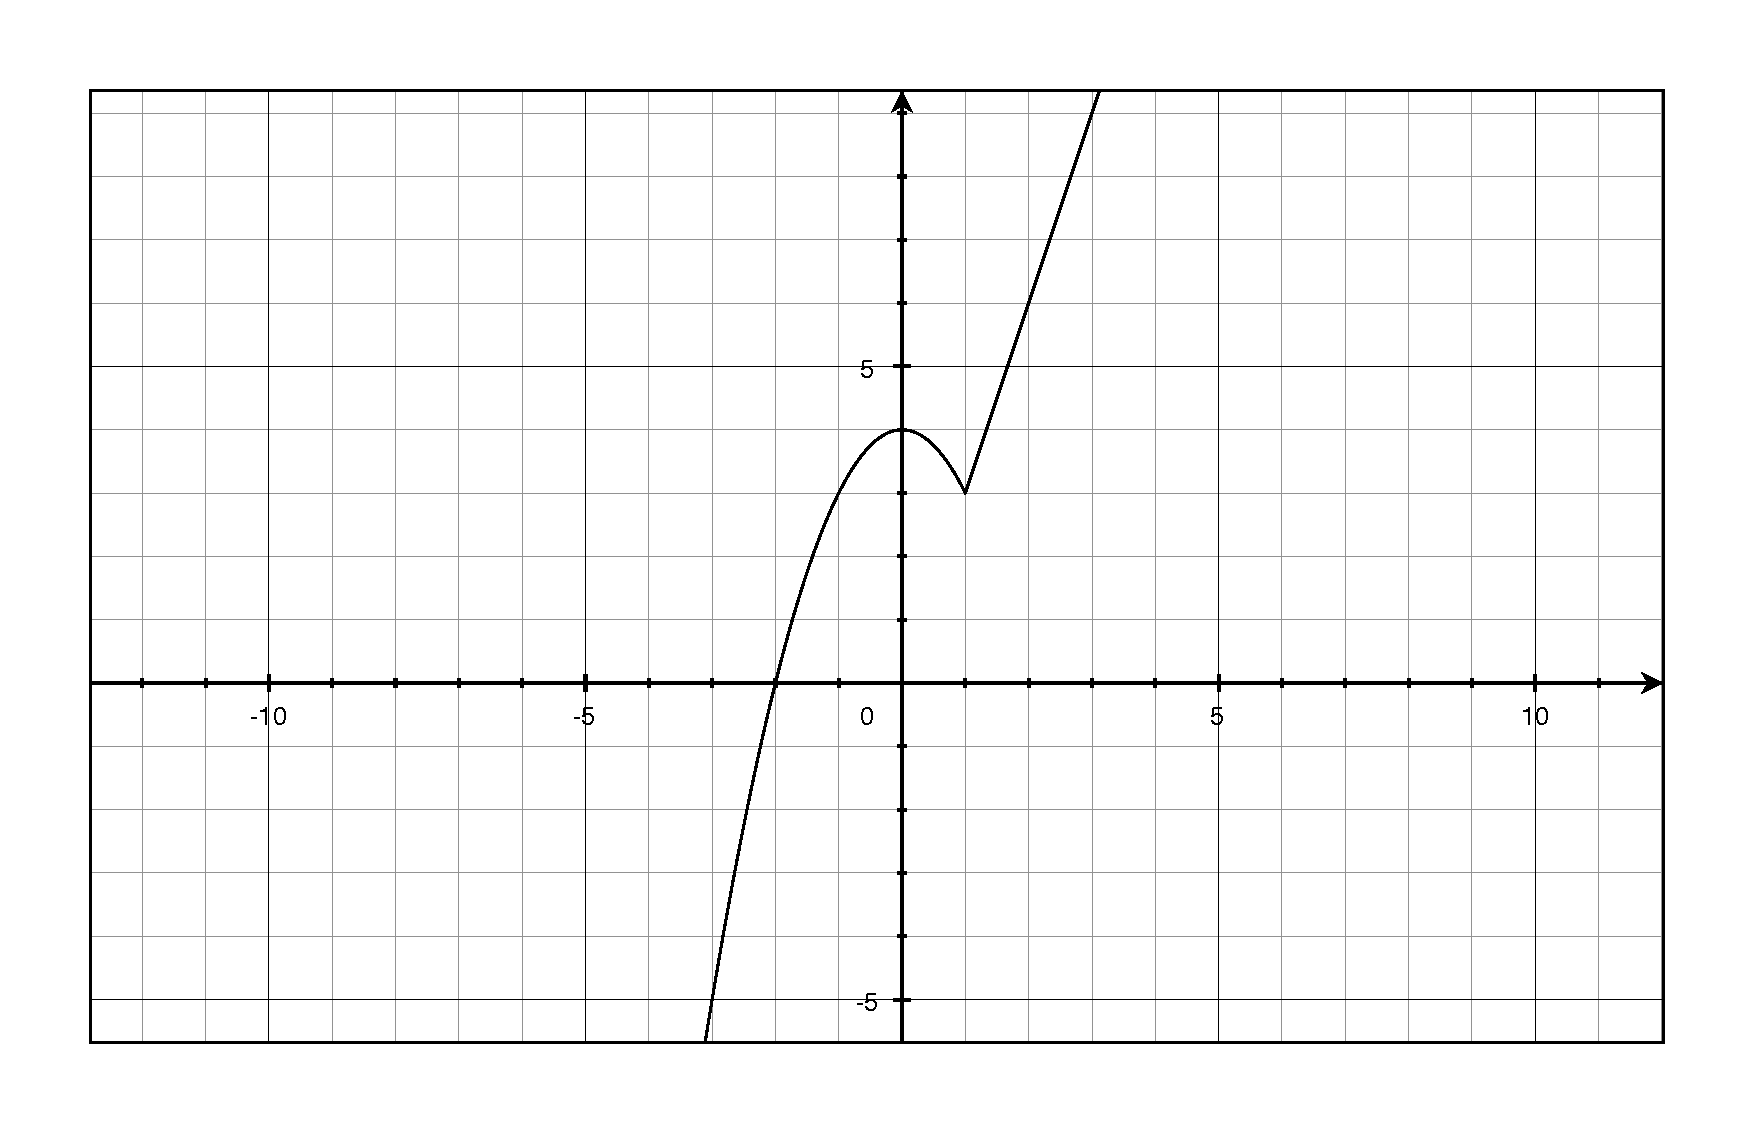
\includegraphics[scale=.3]{question_32.eps}
  \caption*{Question 32}
\end{figure}

\end{description}

\else

\vspace{10 cm}

{\em 

A minority is powerless while it conforms to the majority; it is not even a minority then; but it is irresistible
  when it clogs by its whole weight. If the alternative is to keep all just men in prison, or give up war and slavery,
  the State will not hesitate which to choose. If a thousand men were not to pay their tax-bills this year, that would
  not be a violent and bloody measure, as it would be to pay them, and enable the State to commit violence and shed
  innocent blood. This is, in fact, the definition of a peaceable revolution, if any such is possible.  }

\vspace{.2 cm}

\hspace{1 cm} --Henry David Thoreau

\fi

\end{document}

